\documentclass[tikz,border=6pt]{standalone}
\usepackage[T1]{fontenc}
\usepackage[utf8]{inputenc}
\usepackage{helvet}
\renewcommand{\familydefault}{\sfdefault}
\usepackage{xcolor}
\usetikzlibrary{arrows.meta}
\definecolor{cblue}{HTML}{1F4E79}
\definecolor{cgreen}{HTML}{2E7D32}
\definecolor{cred}{HTML}{C62828}
\definecolor{cgrey}{HTML}{808080}
\definecolor{paleblue}{HTML}{E8F0F8}
\definecolor{palegreen}{HTML}{E8F5E9}
\definecolor{palered}{HTML}{FFEBEE}
\definecolor{palegrey}{HTML}{F5F5F5}
\begin{document}

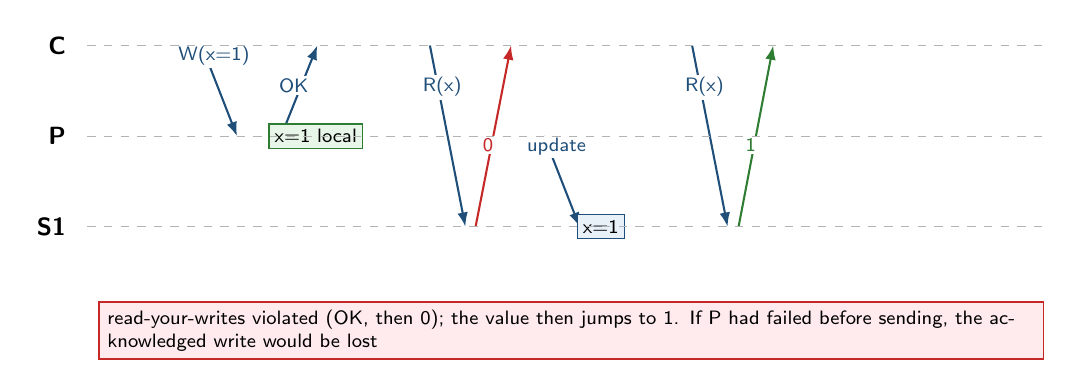
\begin{tikzpicture}[x=1cm,y=1cm]
\draw[-{Latex[length=1.8mm]},cblue,solid,line width=0.75pt] (1.45,0.000) -- (1.90,-1.150) node[pos=0.35,above,yshift=3pt,fill=white,inner sep=1pt,font=\scriptsize] {W(x=1)};
\draw[-{Latex[length=1.8mm]},cblue,solid,line width=0.75pt] (2.46,-1.150) -- (2.92,0.000) node[pos=0.35,above,yshift=3pt,fill=white,inner sep=1pt,font=\scriptsize] {OK};
\node[draw=cgreen,fill=palegreen,line width=0.5pt,inner sep=2pt,font=\scriptsize,align=center] at (2.90,-1.150) {x=1 local};
\draw[-{Latex[length=1.8mm]},cblue,solid,line width=0.75pt] (4.35,0.000) -- (4.80,-2.300) node[pos=0.35,above,yshift=3pt,fill=white,inner sep=1pt,font=\scriptsize] {R(x)};
\draw[-{Latex[length=1.8mm]},cred,solid,line width=0.75pt] (4.93,-2.300) -- (5.38,0.000) node[pos=0.35,above,yshift=3pt,fill=white,inner sep=1pt,font=\scriptsize] {0};
\draw[-{Latex[length=1.8mm]},cblue,solid,line width=0.75pt] (5.80,-1.150) -- (6.25,-2.300) node[pos=0.35,above,yshift=3pt,fill=white,inner sep=1pt,font=\scriptsize] {update};
\node[draw=cblue,fill=paleblue,line width=0.5pt,inner sep=2pt,font=\scriptsize,align=center] at (6.52,-2.300) {x=1};
\draw[-{Latex[length=1.8mm]},cblue,solid,line width=0.75pt] (7.68,0.000) -- (8.13,-2.300) node[pos=0.35,above,yshift=3pt,fill=white,inner sep=1pt,font=\scriptsize] {R(x)};
\draw[-{Latex[length=1.8mm]},cgreen,solid,line width=0.75pt] (8.27,-2.300) -- (8.71,0.000) node[pos=0.35,above,yshift=3pt,fill=white,inner sep=1pt,font=\scriptsize] {1};
\node[anchor=north west,draw=cred,fill=palered,line width=0.5pt,inner sep=3pt,text width=11.78cm,align=left,font=\scriptsize] at (0.14,-3.250) {read-your-writes violated (OK, then 0); the value then jumps to 1. If P had failed before sending, the acknowledged write would be lost};
\draw[cgrey!60,line width=0.4pt,dashed] (0,0.000) -- (12.18,0.000);
\node[anchor=east,font=\small\bfseries] at (-0.15,0.000) {C};
\draw[cgrey!60,line width=0.4pt,dashed] (0,-1.150) -- (12.18,-1.150);
\node[anchor=east,font=\small\bfseries] at (-0.15,-1.150) {P};
\draw[cgrey!60,line width=0.4pt,dashed] (0,-2.300) -- (12.18,-2.300);
\node[anchor=east,font=\small\bfseries] at (-0.15,-2.300) {S1};
\end{tikzpicture}
\end{document}
